L’energia nucleare, oltre che per uccidere migliaia di civili, viene utilizzata per produrre energia elettrica.

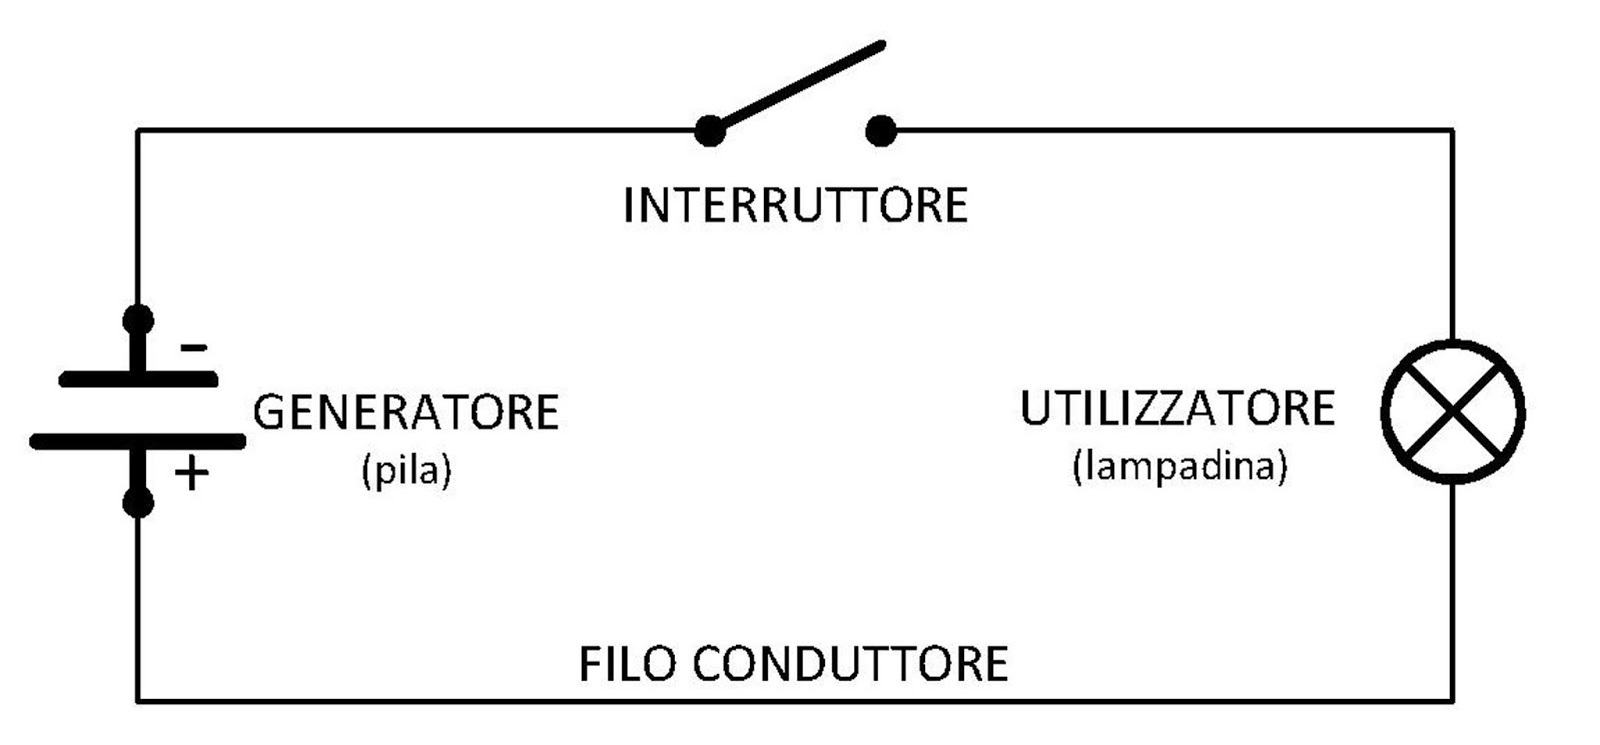
\includegraphics{circuito_elettrico.jpg}

La corrente elettrica è un flusso continuo di elettroni (cariche elettriche) che, attraverso un conduttore, si sposta ordinatamente da un punto di carica negativa (polo negativo) dove si è creato un eccesso di elettroni, a un altro punto di carica positiva (polo positivo) nel quale c’è una carenza di elettroni. Il flusso è costituito di cariche negative e perciò si muove verso il polo positivo: questa è la situazione reale.

L’intensità di corrente è la quantità di corrente che passa attraverso la sezione di un conduttore nell’unità di tempo ed è indicata con il simbolo I. Nel Sistema Internazionale, l’intensità della corrente elettrica si misura in ampere (simbolo A). Lo strumento di misura utilizzato è chiamato amperometro.

La corrente elettrica può essere:
\begin{itemize}
  \item continua se l’intensità e il verso rimangono costanti nel tempo;
  \item alternata se l’intensità e il verso cambiano periodicamente.
\end{itemize}

L’intensità di corrente elettrica è condizionata dalla differenza di carica elettrica esistente tra gli estremi del conduttore e dalla resistenza che il materiale di cui è fatto il conduttore oppone al suo passaggio. Questa differenza si chiama differenza di potenziale(d.d.p.) o in genere tensione elettrica , ed è indicata con il simbolo V. Tanto maggiore è la differenza di potenziale elettrico tanto maggiore è l’intensità di corrente a parità di resistenza. Nel SI, la differenza di potenziale si misura in volt (V) e lo strumento di misura utilizzato si chiama voltmetro.

I conduttori non trasportano la corrente tutti allo stesso modo ma offrono a essa una resistenza a farsi attraversare dalla corrente diversa. Il valore della resistenza dipende:
\begin{itemize}
  \item Dalle caratteristiche del materiale utilizzato per realizzare il conduttore;
  \item Dalla sezione del conduttore: la resistenza di un conduttore diminuisce all’aumentare della sua sezione.
\end{itemize}
La resistenza elettrica viene indicata con il simbolo R e si misura in ohm.
